\documentclass{article}

\usepackage[paperwidth=78in,paperheight=30in,margin=0.75in]{geometry}
\usepackage{amsmath,amssymb}
\usepackage{booktabs}
\usepackage[most]{tcolorbox}
\usepackage{graphicx}
\usepackage{xcolor}
\usepackage{multicol}
\usepackage{array}
\usepackage{url}
\pagestyle{empty}

\graphicspath{{figures/}}

\definecolor{ink}{HTML}{102A43}
\definecolor{muted}{HTML}{52616B}
\definecolor{blue}{HTML}{2F4B7C}
\definecolor{green}{HTML}{00A676}
\definecolor{orange}{HTML}{F28E2B}
\definecolor{panel}{HTML}{F7FAFC}
\definecolor{line}{HTML}{D9E2EC}

\newtcolorbox{posterbox}[2][]{
  enhanced,
  colback=white,
  colframe=#2,
  boxrule=3pt,
  arc=8pt,
  left=18pt,
  right=18pt,
  top=16pt,
  bottom=16pt,
  title=#1,
  coltitle=ink,
  fonttitle=\bfseries\fontsize{34}{38}\selectfont,
  attach boxed title to top left={xshift=18pt,yshift=-10pt},
  boxed title style={colback=white,colframe=white}
}

\newcommand{\metric}[3]{%
\begin{tcolorbox}[enhanced,colback=#1!8,colframe=#1,boxrule=2.5pt,arc=8pt,width=0.31\linewidth,halign=center,valign=center]
{\fontsize{42}{46}\selectfont\bfseries #2}\\[6pt]
{\fontsize{20}{24}\selectfont #3}
\end{tcolorbox}}

\begin{document}
\color{ink}

\begin{tcolorbox}[enhanced, colback=ink, colframe=ink, arc=0pt, boxrule=0pt, left=30pt, right=30pt, top=28pt, bottom=28pt]
{\color{white}\fontsize{76}{82}\selectfont\bfseries Cost-Aware Conditional Diffusion Compression of 4K-5K Drone Imagery}\\[14pt]
{\color{white}\fontsize{34}{40}\selectfont Jooho Kim, Anish Shakya, Yifan Yang, and Jacob Kelly \hfill Texas A\&M University}
\end{tcolorbox}

\vspace{0.45in}

\begin{minipage}[t]{0.31\linewidth}
\vspace{0pt}
\begin{posterbox}[Problem]{blue}
{\fontsize{25}{31}\selectfont
Post-disaster drone flights produce high-resolution imagery that is useful for inspection, mapping, and damage assessment. The cost appears downstream: full-resolution diffusion decoding moves slowly, uses large GPU memory, and makes repeated HPC workflows expensive. We ask a systems question: which operating point keeps native visual detail while reducing runtime and memory?}
\end{posterbox}

\vspace{0.35in}
\begin{posterbox}[Decision Equations]{green}
{\fontsize{28}{36}\selectfont
\[
R=\frac{24}{\mathrm{BPP}}
\]
\[
S_T=1-\frac{T_{\mathrm{tile}}}{T_{\mathrm{full}}},\qquad
G_M=\frac{M_{\mathrm{full}}}{M_{\mathrm{tile}}}
\]
\[
C(\theta)=\alpha \hat{T}+\beta \hat{M}+\gamma(1-\mathrm{SSIM})
\]
The score is a transparent decision aid, not a universal model metric.}
\end{posterbox}

\vspace{0.35in}
\begin{posterbox}[Key Result]{orange}
\noindent
\metric{green}{44.7\%}{runtime reduction}\hfill
\metric{blue}{31.3$\times$}{lower peak memory}\hfill
\metric{orange}{0.0031}{SSIM drop vs 512 tile}
{\fontsize{25}{31}\selectfont
The selected $256 \times 256$ tile is the current speed and memory candidate. It preserves the native image boundary and lowers peak memory from 52.01 GB to 1.66 GB on 50 full-resolution images.}
\end{posterbox}
\end{minipage}
\hfill
\begin{minipage}[t]{0.36\linewidth}
\vspace{0pt}
\begin{posterbox}[Cost-Memory-Quality Dashboard]{green}
\centering
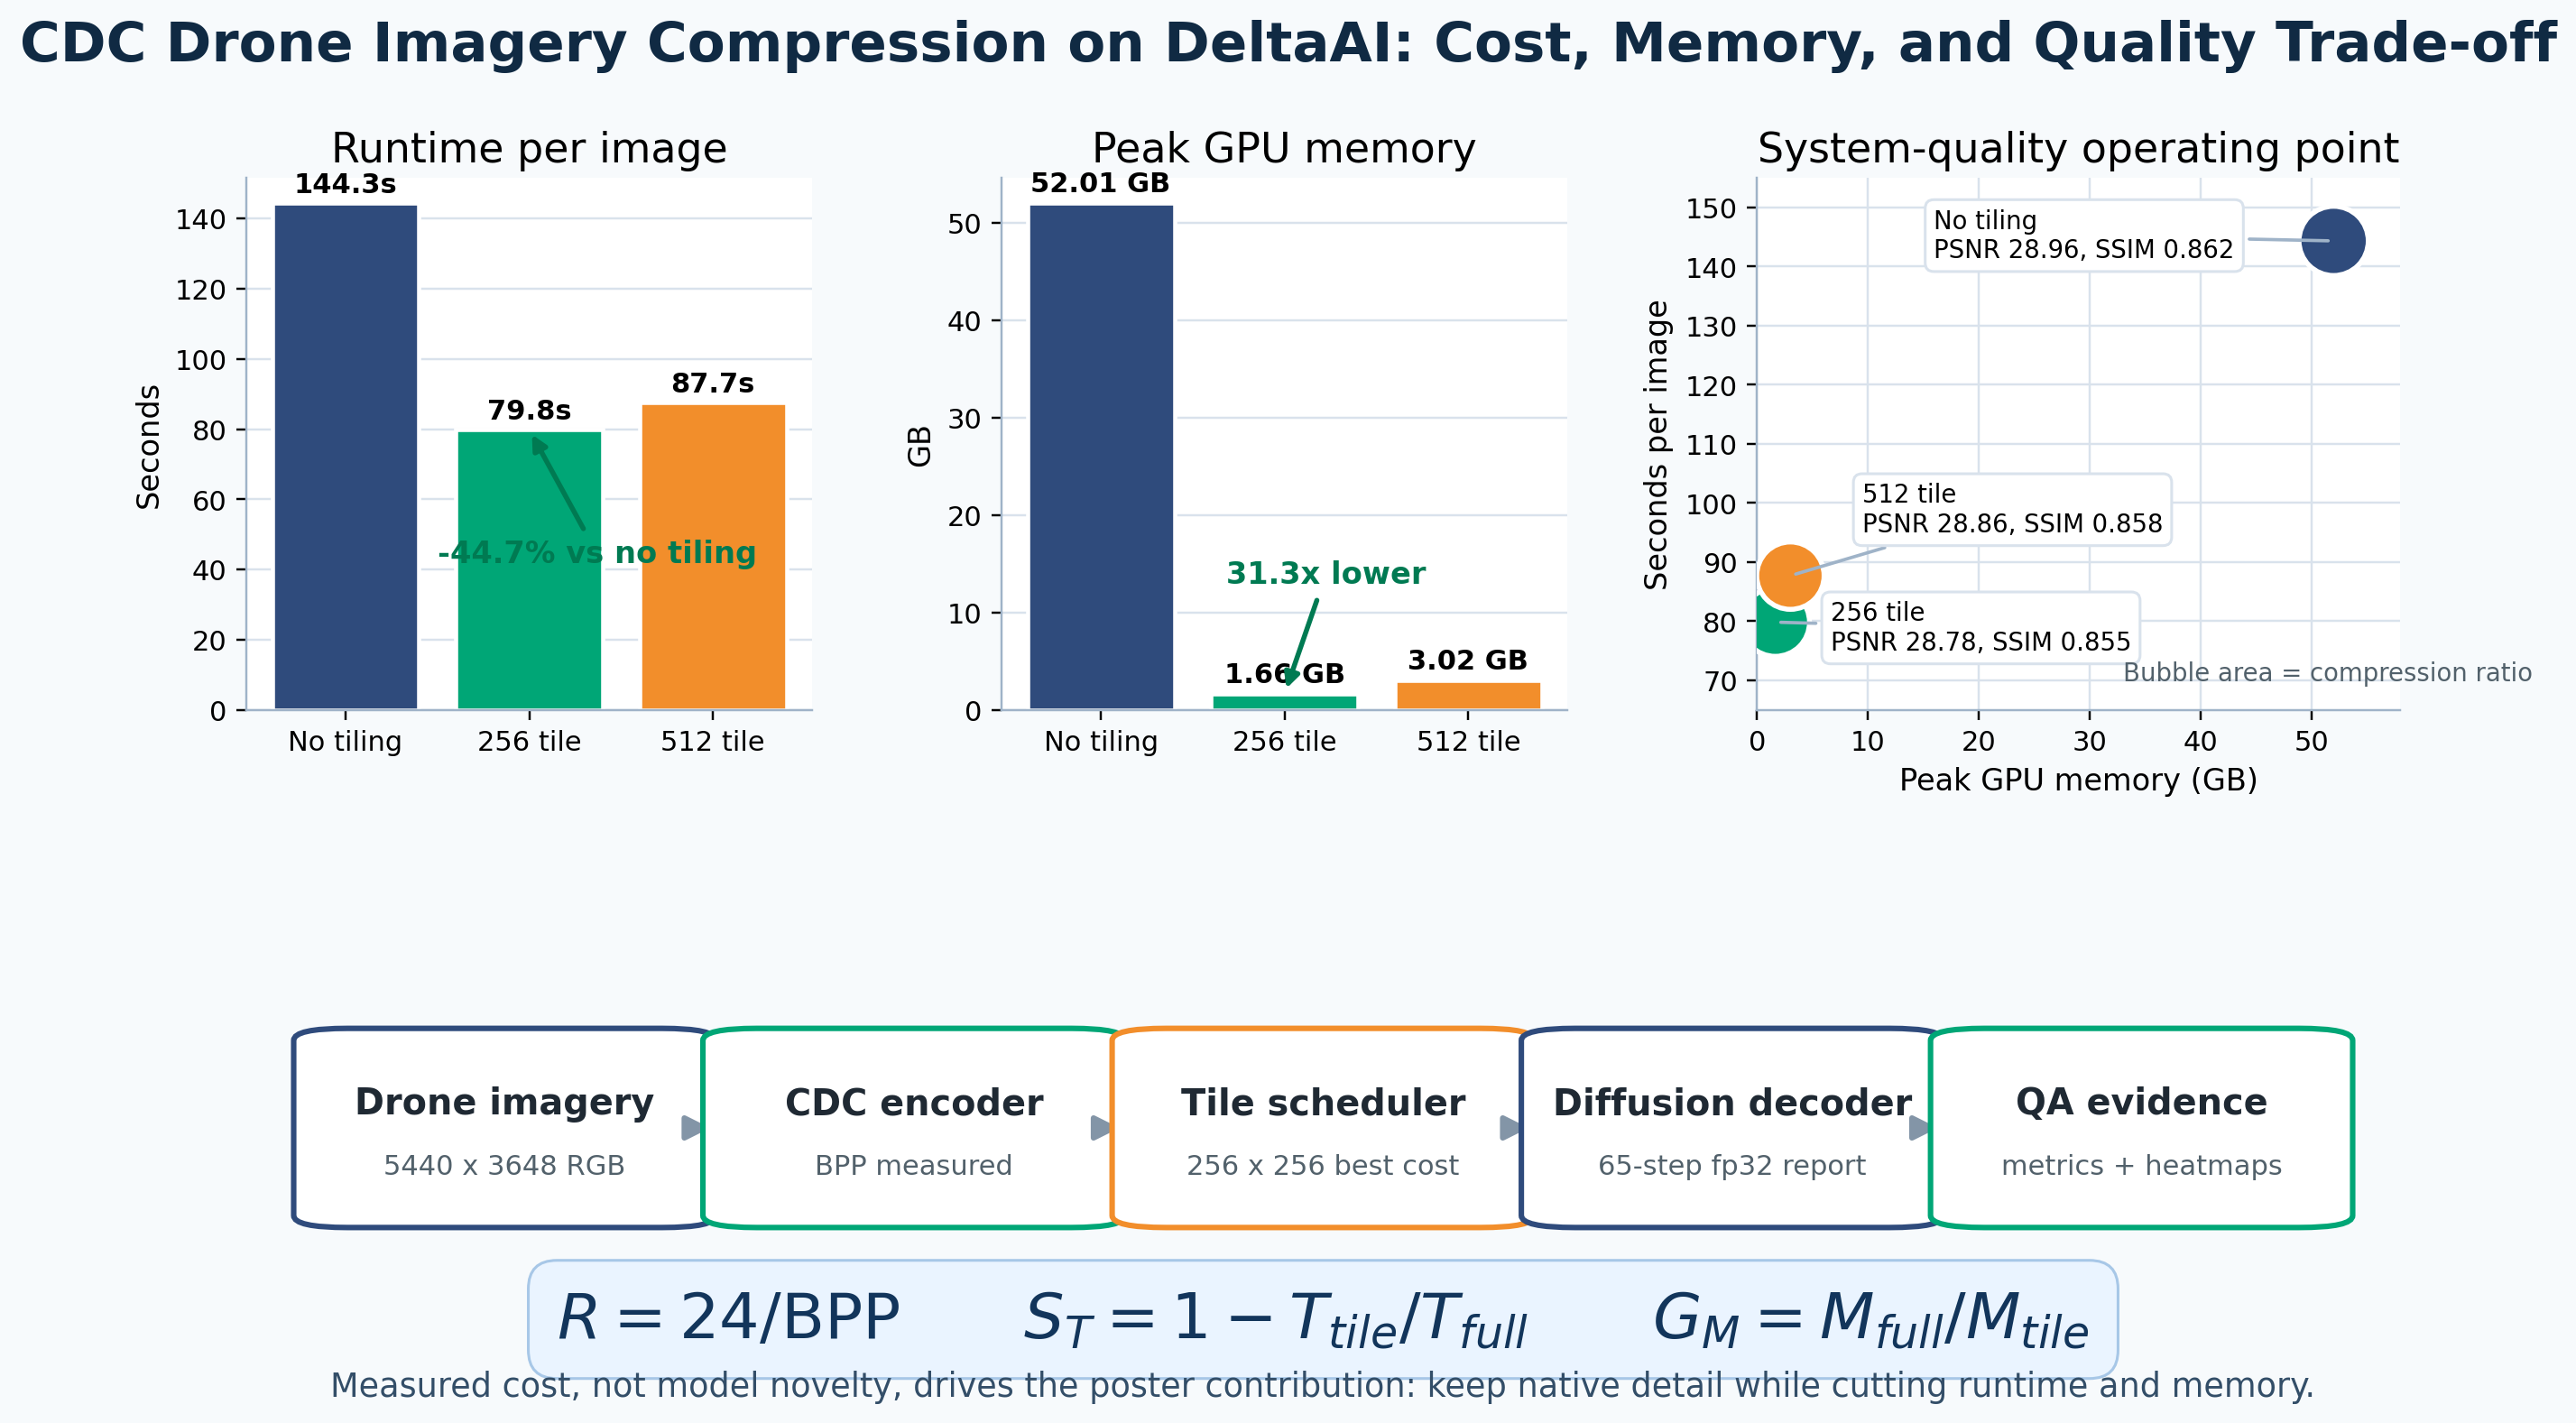
\includegraphics[width=\linewidth]{tradeoff_dashboard.png}
\end{posterbox}

\vspace{0.35in}
\begin{posterbox}[Selected Validation Table]{blue}
\centering
{\fontsize{24}{30}\selectfont
\begin{tabular}{lrrrrr}
\toprule
Setup & Sec./img & GPU GB & Ratio & PSNR & SSIM\\
\midrule
No tiling & 144.35 & 52.01 & 70.11$\times$ & 28.96 & 0.8616\\
$256^2$ tile & 79.84 & 1.66 & 68.24$\times$ & 28.78 & 0.8552\\
$512^2$ tile & 87.71 & 3.02 & 66.31$\times$ & 28.86 & 0.8583\\
\bottomrule
\end{tabular}}
\end{posterbox}
\end{minipage}
\hfill
\begin{minipage}[t]{0.29\linewidth}
\vspace{0pt}
\begin{posterbox}[Visual QA Evidence]{orange}
\centering

\includegraphics[width=\linewidth]{tile256_poster_panel.jpg}
\vspace{0.15in}
{\fontsize{21}{27}\selectfont
The poster keeps visual evidence next to scalar metrics. The QA panel combines original preview, reconstruction, hot difference map, pixel-error histogram, metric block, and difference distribution.}
\end{posterbox}

\vspace{0.35in}
\begin{posterbox}[Interpretation]{blue}
{\fontsize{25}{31}\selectfont
\textbf{1. Native full-image CDC is feasible but memory-heavy.}\\
Baseline decoding takes about 144 seconds per image and peaks near 52 GB.\\[10pt]
\textbf{2. Resolution reduction is fast but quality-limited.}\\
2K inputs run quickly, but SSIM drops to about 0.689.\\[10pt]
\textbf{3. Tiling is the practical control.}\\
$256 \times 256$ tiling gives the strongest measured runtime and memory improvement with small scalar quality loss.\\[10pt]
\textbf{Next update.} Add a larger validation run, more visual panels, and downstream disaster-analysis checks.}
\end{posterbox}
\end{minipage}

\vspace{0.45in}

\begin{minipage}[t]{0.31\linewidth}
\vspace{0pt}
\begin{posterbox}[Experiment Matrix]{green}
{\fontsize{24}{30}\selectfont
\textbf{Controls tested:} native full-resolution decoding, resolution reduction, denoising steps, tile size, checkpoint choice, batch size, storage placement, and parallel shards.\\[8pt]
\textbf{Primary measured quantities:} seconds per image, peak GPU memory, BPP, compression ratio, PSNR, SSIM, MAE, error p99, and seam metrics.}
\end{posterbox}
\end{minipage}
\hfill
\begin{minipage}[t]{0.36\linewidth}
\vspace{0pt}
\begin{posterbox}[Why This Belongs at SC]{blue}
{\fontsize{24}{30}\selectfont
The contribution is an HPC operating-point study: the same CDC model can be impractical or usable depending on GPU memory pressure, diffusion runtime, and image tiling. The poster reports model quality together with system cost, so reviewers can see the path from algorithm to deployable disaster-imagery workflow.}
\end{posterbox}
\end{minipage}
\hfill
\begin{minipage}[t]{0.29\linewidth}
\vspace{0pt}
\begin{posterbox}[Final-Version Updates]{orange}
{\fontsize{24}{30}\selectfont
Before final upload: add a larger selected run, more representative visual QA panels, downstream disaster-analysis checks, and a QR code linking to code, result tables, and a short video explanation.}
\end{posterbox}
\end{minipage}

\vfill
{\fontsize{19}{23}\selectfont\color{muted}
Context: this project connects HPC compression with disaster-imagery workflows, including Satellite-to-Street generative views and hyperlocal street-view damage assessment. Code and lightweight result artifacts remain in \texttt{rayford295/sc26-cdc-deltaai}; raw images and full DeltaAI outputs stay off GitHub.}

\end{document}
